% !TEX root = main.tex

\subsection{Comparison to the Electricity Mix}
\label{ch:elecMix}

Comparing the emission factor with the emission factors of the electricity mix of other countries enables us to identify where technologies like the ASF would be best suited. In Switzerland where the simulation was run, we see a 6\% reduction compared to the average electricity mix. This is because the Swiss electricity mix is dominated by Hydro and Nuclear which has a very low GWP potential. In Germany on the other hand, the ASF has a 81\% reduction in carbon emissions. \\

\begin{figure}[H]
\begin{center}
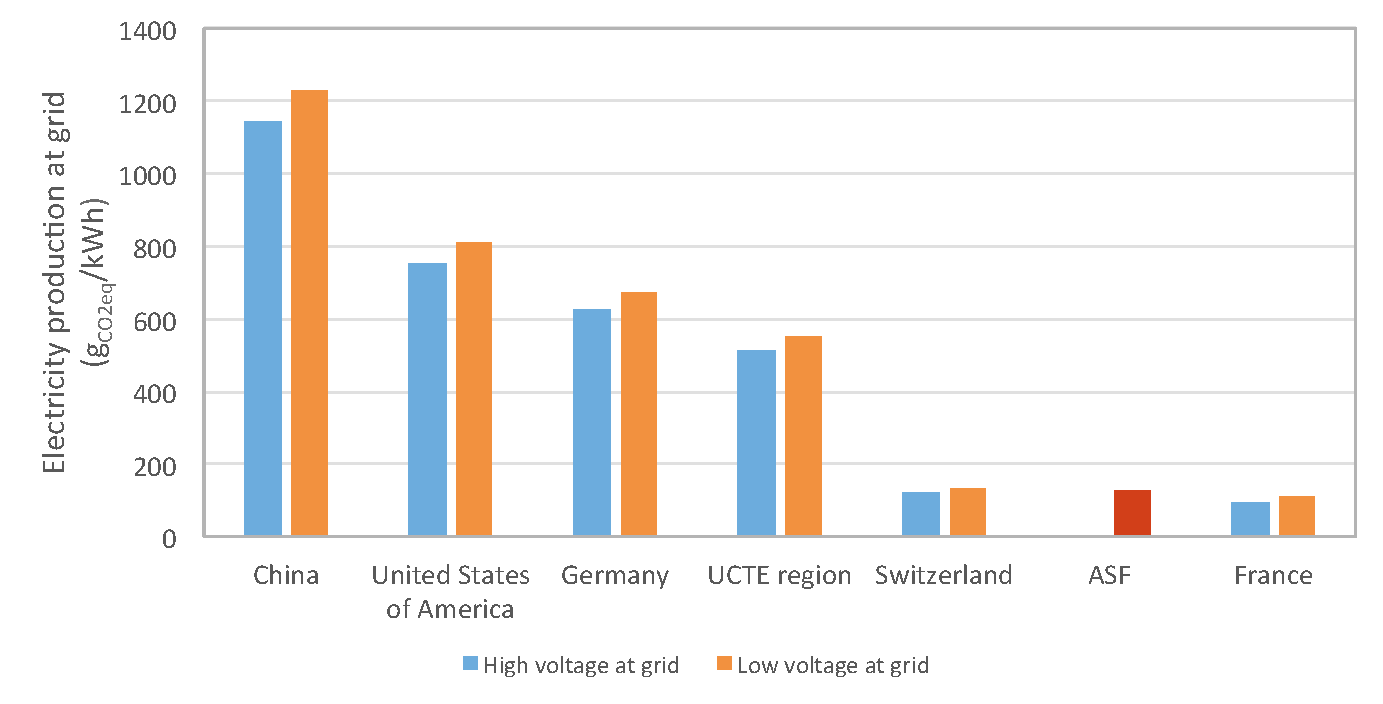
\includegraphics[width=10cm, trim= 0cm 0cm 0cm 0cm,clip]{regionGridMix.pdf}
\caption{Comparison of the ASF when in operated in Switzerland when compared to other countries in the world that have similar climate conditions. Note that the data will have to change because we can't really compare (ASF in Switzerland) with Germany. We should be comparing the ASF in Germany with Germany}
\label{fig:compReg}
\end{center}
\end{figure}


\subsection{Comparison to other technologies}

Comparison of the ASF to other PV technologies and the UCTE electricity mix is highlighted in Figure \ref{fig:compPV}. We can see in this figure that the ASF without shading benefits is inferior to all other technologies. It is only with the added shading benefits that we really see the advantages of the adaptive system.
We can also see that the utilisation of the ASF in an area where the electricity mix has low GWP intensity such as Switzerland also has disadvantages. It is capable of out performing Silicone based technologies but is still inferior to simply mounted CIGS panels. Note that even the panels themselves of the ASF, without the BOS, is still lower that the CIGS installation. This is due to the added inefficiencies as the panels are not always at the optimum position to the sun.


\begin{figure}[H]
\begin{center}
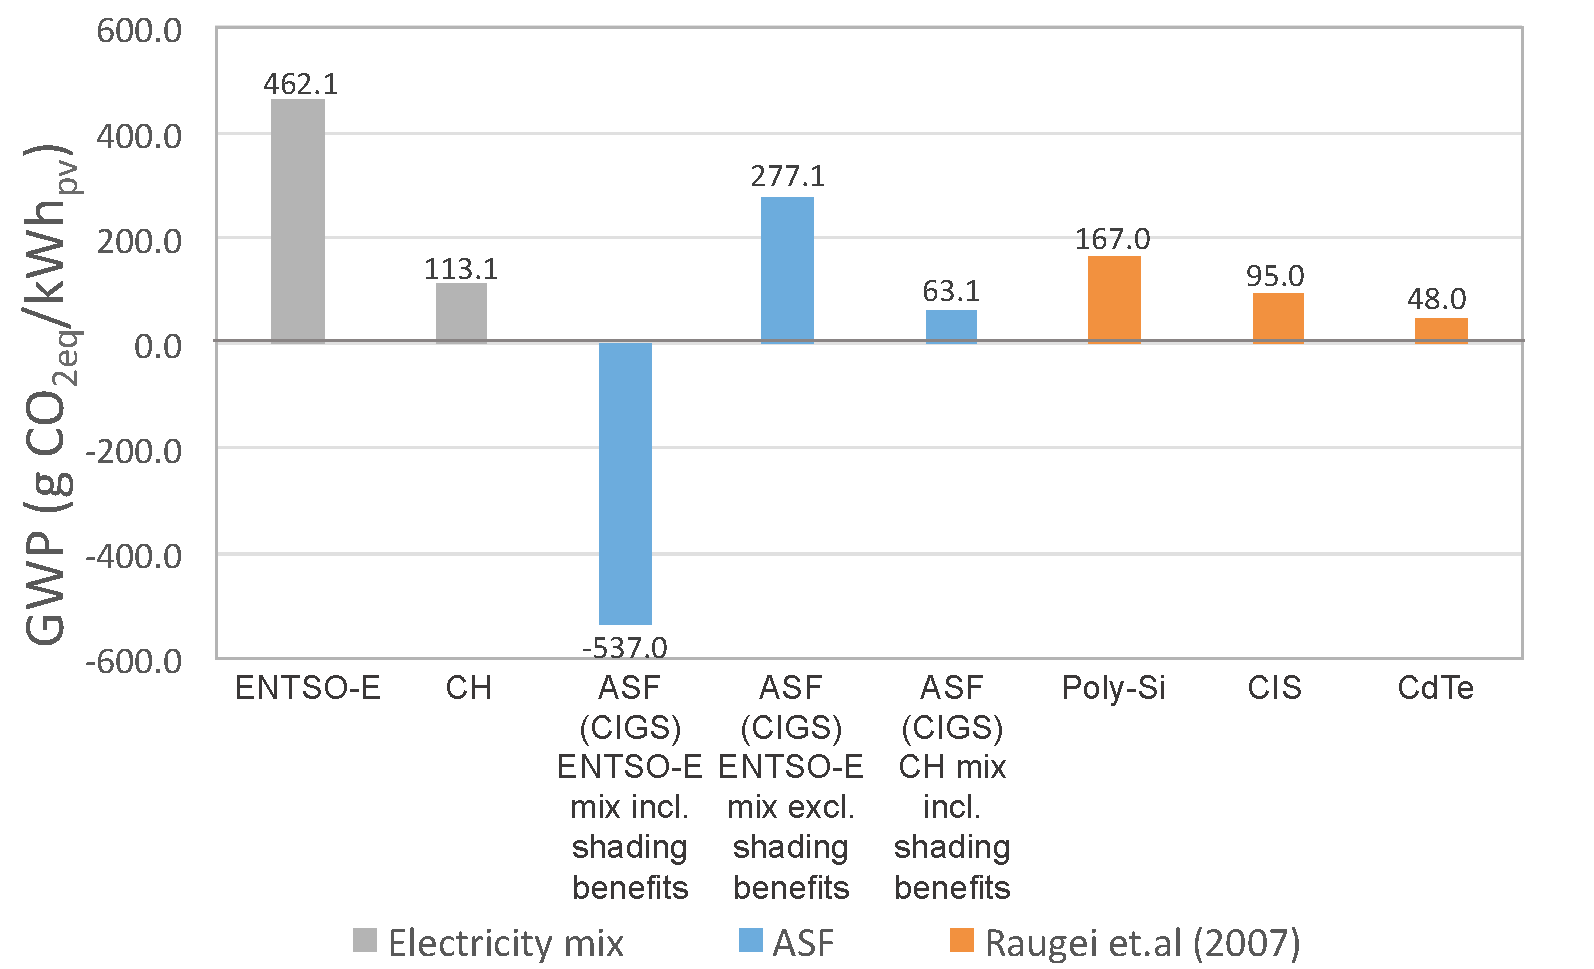
\includegraphics[width=10cm, trim= 0cm 0cm 0cm 0cm,clip]{compPV.pdf}
\caption{Comparison of thin-film and BOS to other PV technologies. I would add some extra columns, one without shading, one with the ASF in Switzerland, one with the ASF in Europe}
\label{fig:compPV}
\end{center}
\end{figure}

The comparison of the ASF to a simple shading system shows...


\begin{figure}[H]
\begin{center}
\includegraphics[width=10cm, trim= 0cm 0cm 0cm 0cm,clip]{louvres}
\caption{The comparison of the ASF with a static louvered shading system. Staked bar plots may be better}
\label{fig:louvres}
\end{center}
\end{figure}
% I think I would prefer good old stacked bar plots


